\documentclass[UTF8,a4paper]{article}
\usepackage{ctex}
\usepackage{amsmath}
\usepackage{amssymb}
\usepackage{graphicx}
\usepackage{fancyhdr}
\usepackage{CJK}
\usepackage{chngpage}
\usepackage{url}
\setCJKmainfont{宋体}
\usepackage{listings}
\usepackage{xcolor}
\usepackage[numbers,sort&compress]{natbib}
\usepackage{xpatch}
\usepackage{geometry}
\xpatchcmd{\thebibliography}{\section*}{\section}{}{}
\geometry{left=2.9cm,right=2.9cm,top=3cm,bottom=2.9cm}

\definecolor{CPPLight}  {HTML} {686868}
\definecolor{CPPSteel}  {HTML} {888888}
\definecolor{CPPDark}   {HTML} {262626}
\definecolor{CPPBlue}   {HTML} {4172A3}
\definecolor{CPPGreen}  {HTML} {487818}
\definecolor{CPPBrown}  {HTML} {A07040}
\definecolor{CPPRed}    {HTML} {AD4D3A}
\definecolor{CPPViolet} {HTML} {7040A0}
\definecolor{CPPGray}  {HTML} {B8B8B8}


\lstset{
	columns=fixed,       
	numbers=left,                                        % 在左侧显示行号
	frame=none,                                          % 不显示背景边框
	backgroundcolor=\color[RGB]{245,245,244},            % 设定背景颜色
	keywordstyle=\color[RGB]{40,40,255},                 % 设定关键字颜色
	numberstyle=\footnotesize\color{darkgray},           % 设定行号格式
	commentstyle=\it\color[RGB]{0,96,96},                % 设置代码注释的格式
	basicstyle=\small,
	stringstyle=\rmfamily\slshape\color[RGB]{128,0,0},   % 设置字符串格式
	showstringspaces=false,                              % 不显示字符串中的空格
	language=c++,                                        % 设置语言
	morekeywords={alignas,continute,friend,register,true,alignof,decltype,goto,
		reinterpret_cast,try,asm,defult,if,return,typedef,auto,delete,inline,short,
		typeid,bool,do,int,signed,typename,break,double,long,sizeof,union,case,
		dynamic_cast,mutable,static,unsigned,catch,else,namespace,static_assert,using,
		char,enum,new,static_cast,virtual,char16_t,char32_t,explict,noexcept,struct,
		void,export,nullptr,switch,volatile,class,extern,operator,template,wchar_t,
		const,false,private,this,while,constexpr,float,protected,thread_local,
		const_cast,for,public,throw,std},
	emph={map,set,multimap,multiset,unordered_map,unordered_set,
		unordered_multiset,unordered_multimap,vector,string,list,deque,
		array,stack,forwared_list,iostream,memory,shared_ptr,unique_ptr,
		random,bitset,ostream,istream,cout,cin,endl,move,default_random_engine,
		uniform_int_distribution,iterator,algorithm,functional,bing,numeric,},
	emphstyle=\color{CPPViolet}, 
}



%opening
\title{实验五 数字签字算法DSA}
\author{1611531-信息安全-刘新慧}
\date{}
\begin{document}

\maketitle

\begin{abstract}
通过对数字签字算法DSA的实际操作,理解DSS的基本工作原理。\par 
\end{abstract}
\tableofcontents
\newpage
	\section{实验内容和步骤}
1、	为了加深对RSA算法的了解,根据已知参数:p=3,q=11,m=2,
手工计算公钥和私钥,并对明文m进行加密,然后对密文进行解密。\par 
2、编写一个程序,用于生成512比特的素数。\par 
3.	利用2中程序生成的素数,构建一个n的长度为1024比特的RSA算法,
利用该算法实现对明文的加密和解密。\par 
4、在附件中还给出了一个可以进行RSA加密和解密的对话框程序RSATool,运行这个程序加密一段文字,了解RSA算法原理。\par 

	\section{实验原理}
	\subsection{DSA原理}
以往的文件或书信可以通过手写亲笔签名来证明其真实性,而通过计算机网络传输的信息则通过数字签字技术实现其真实性的验证。\par 
数字签字目前采用较多的是非对称加密技术,其实现原理简单的说,就是由发送方利用杂凑函数对要传送的信息进行计算得到一个固定位数的消息摘要值,用发送者的私钥加密此消息的杂凑值所产生的密文即数字签字。然后将数字签字和消息一同发送给接收方。接收方收到消息和数字签字后,用同样的杂凑函数对消息进行计算得到新的杂凑值,然后用发送者的公开密钥对数字签字解密,将解密后的结果与自己计算得到的杂凑值相比较,如相等则说明消息确实来自发送方。\par 
下面我们以DSA(Digital Signature Algorithm)为例,介绍数字签字算法。DSA源于Elgamal签名算法,被美国NIST采纳为DSS(Digital Signature Standard)数字签名标准。下面介绍DSA的算法描述:\par 

1.	全局变量的设置\par 
(1)	素数p,$2^{511}<p<2^{512}$;\par 
(2)	q是p-1的一个素因子,$2^{159}<q<2^{160}$;\par 
(3)	 其中h是整数,1<h<(p-1).\par 
2.	私钥:\par 
私钥x是随机数或伪随机数,其中0<x<q.\par 
3. 公钥:\par 
y=$g^{x}$mod p,(p,q,g,y)为公钥。\par 
4.用户的随机数选择:\par 
k为随机数或伪随机数,其中0<k<q。\par 
基于以上选择的参数,DSA的签字过程如下:\par 
\begin{center}
	$\gamma =(g^k mod p)mod q$\par 
	
	$\delta =(k^{-1}(H(m)+xr))mod q$\par 
\end{center}
 则$(\gamma,\delta)$为对消息m的签字,显然,签字长度为320比特。\par 
其中,H是一个安全杂凑函数,在DSS标准中,采用SHA-1算法作为安全的杂凑函数。\par 
签字完成后,把对消息m的数字签字 和消息m一同发送给接收方。接收方接收到消息m和数字签字 后,对数字签字的验证过程如下:\par 
 计算:\par 

\begin{center}
	$w=\delta ^{-1} mod q$\par 
	
	$\u1=H(m)w mod q$\par 
	$\u2=\gamma w mod q$\par 
\end{center}
 如果有: $((g^{u1}y^{u2})mod p)mod q=\gamma$ ,则说明信息确实来自发送方。否则,签字是无效的。\par 




\subsection{杂凑函数SHA}
SHA-1算法是SHA 家族成员之一。


SHA (Secure Hash Algorithm,译作安全散列算法) 是美国国家安全局 (NSA) 设计,美国国家标准与技术研究院(NIST) 发布的一系列密码散列函数。正式名称为 SHA 的家族第一个成员发布于 1993年。然而人们给它取了一个非正式的名称 SHA-0 以避免与它的后继者混淆。两年之后, SHA-1,第一个 SHA 的后继者发布了。 另外还有四种变体,曾经发布以提升输出的范围和变更一些细微设计: SHA-224, SHA-256, SHA-384 和 SHA-512 (这些有时候也被称做 SHA-2)。


最初载明的算法于1993年发布,称做安全散列标准 (Secure Hash Standard),FIPS PUB 180。这个版本常被称为 "SHA-0"。它在发布之后很快就被NSA撤回,并且以 1995年发布的修订版本 FIPS PUB 180-1 (通常称为 "SHA-1") 取代。根据 NSA的说法,它修正了一个在原始算法中会降低密码安全性的错误。然而 NSA 并没有提供任何进一步的解释或证明该错误已被修正。1998年,在一次对 SHA-0 的攻击中发现这次攻击并不能适用于 SHA-1 — 我们不知道这是否就是NSA 所发现的错误,但这或许暗示我们这次修正已经提升了安全性。SHA-1已经被公众密码社群做了非常严密的检验而还没发现到有不安全的地方,它被认为是安全的。


SHA-0 和 SHA-1 会从一个最大 2\^{}64 位元的讯息中产生一串 160 位元的摘要,然后以设计 MD4 及 MD5 讯息摘要算法的 MIT 教授Ronald L. Rivest类似的原理为基础来加密。


SHA-1 的描述:


以下是 SHA-1 算法的伪代码:




\begin{lstlisting}[language = C++, numbers=left, 
numberstyle=\tiny,keywordstyle=\color{blue!70},
commentstyle=\color{red!50!green!50!blue!50},frame=shadowbox,
rulesepcolor=\color{red!20!green!20!blue!20},basicstyle=\small\ttfamily]
(Initialize variables:)
a = h0 = 0x67452301
b = h1 = 0xEFCDAB89
c = h2 = 0x98BADCFE
d = h3 = 0x10325476
e = h4 = 0xC3D2E1F0
(Pre-processing:)
paddedmessage = (message) append 1
while length(paddedmessage) mod 512 <> 448:
paddedmessage = paddedmessage append 0
paddedmessage = paddedmessage append (length(message) in 64-bit format)
(Process the message in successive 512-bit chunks:)
while 512-bit chunk(s) remain(s):
break the current chunk into sixteen 32-bit words w(i), 0 <= i <= 15
(Extend the sixteen 32-bit words into eighty 32-bit words:)
for i from 16 to 79:
w(i) = (w(i-3) xor w(i-8) xor w(i-14) xor w(i-16)) leftrotate 1
(Main loop:)
for i from 0 to 79:
temp = (a leftrotate 5) + f(b,c,d) + e + k + w(i) (note: all addition is mod 2^32)
where:
(0 <= i <= 19): f(b,c,d) = (b and c) or ((not b) and d), k = 0x5A827999
(20 <= i <= 39): f(b,c,d) = (b xor c xor d), k = 0x6ED9EBA1
(40 <= i <= 59): f(b,c,d) = (b and c) or (b and d) or (c and d), k = 0x8F1BBCDC
(60 <= i <= 79): f(b,c,d) = (b xor c xor d), k = 0xCA62C1D6
e = d
d = c
c = b leftrotate 30
b = a
a = temp
h0 = h0 + a
h1 = h1 + b
h2 = h2 + c
h3 = h3 + d
h4 = h4 + e
digest = hash = h0 append h1 append h2 append h3 append h4

\end{lstlisting}\par 
在FIPS PUB 180-1 展示的构想,用以下的公式替代可以增进效能:\par 
\begin{center}
	(0 <= i <= 19):$ 
	F(B,C,D)=D\oplus (B\wedge(C\oplus D))
	$\par 	
	
	(40 <= i <= 59):$ 
	F(B,C,D)=(B\wedge C)\vee(D\wedge(B\vee C))
	$\par 
\end{center}
SHA-1 在许多安全协议中广为使用,包括TLS 和SSL、PGP、SSH、S/MIME
和IPsec,曾被视为是MD5(更早之前被广为使用的散列函数)的后继者。\par 


	\subsection{SHA与MD5比较}


1 对强行攻击的安全性;最显著和重要的区别是SHA-1摘要长32位,使用强行技术.产生任何一个报文使其摘要等于给报摘要的难度对MD5是\^{}128数量级的操作,而对SHA-1则是2\^{}160数量级的操作,这样,SHA-1对强行攻击 有更大的强度, 


2 对密码分析的安全性:由于MD5的设计.易受密码分析的攻击,SHA-1显得不容易受这样的攻击. 


3 速度:在相同的硬件上,SHA-1的运行速度比MD5慢.









\section{程序演示}

打开程序运行,通过移动鼠标获得种子进而生成DSA数字签名算法的全局公开钥p,q,g以及用户公开钥y,用户私密钥x。\par \newpage
\begin{figure}[!ht]
	
	\centering
	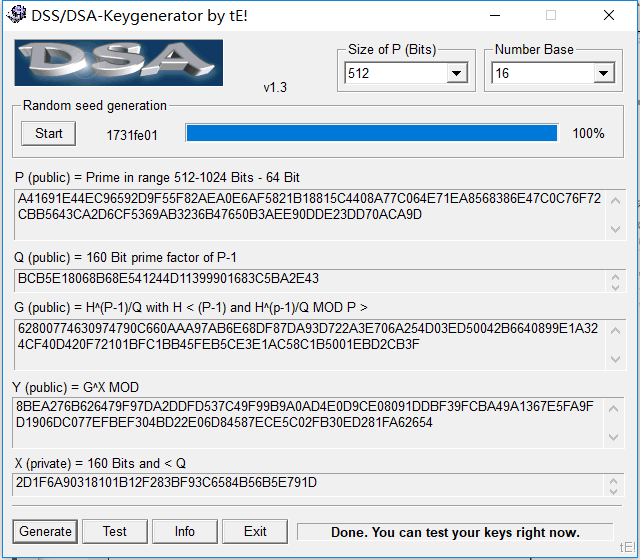
\includegraphics[width=0.67\textwidth]{pic1.PNG}
	\caption{获得种子}
	\label{fig:1-1}
\end{figure}
对消息进行签名:\par 
\begin{figure}[!ht]
	
	\centering
	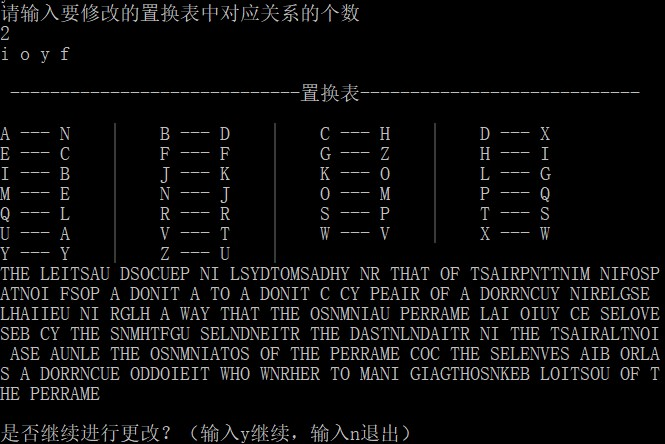
\includegraphics[width=0.67\textwidth]{pic2.PNG}
	\caption{进行签名}
	\label{fig:1-1}
\end{figure}

进行验证,消息正确则验证成功,消息错误则验证失败。\par 
\begin{figure}[!ht]
	
	\centering
	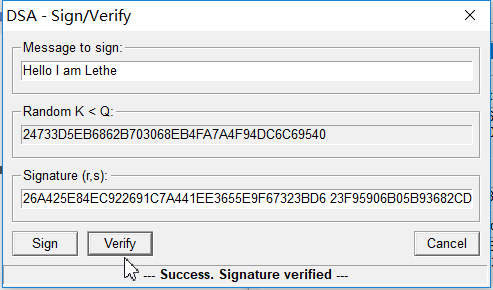
\includegraphics[width=0.67\textwidth]{pic3.PNG}
	\caption{验证成功}
	\label{fig:1-1}
\end{figure}


\begin{figure}[!ht]
	
	\centering
	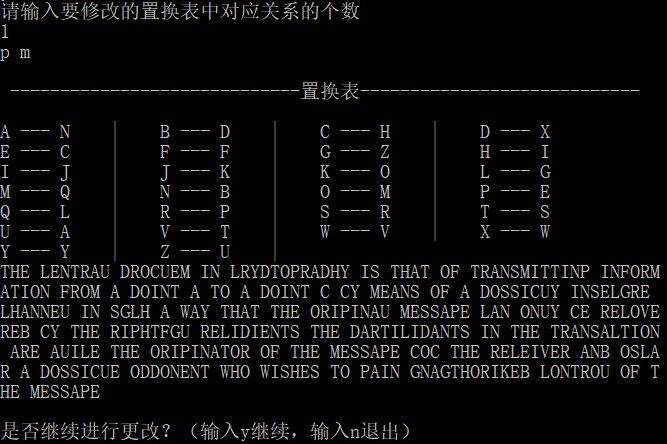
\includegraphics[width=0.67\textwidth]{pic4.PNG}
	\caption{验证失败}
	\label{fig:1-1}
\end{figure}



\end{document}
